\part{Optimalizace orientace faset}
	
\section{Schéma optimalizačního procesu}

%Přecházíme k situaci, kdy máme dostupné informace o simulovaných i pozorovaných svazcích. Mezi těmito dvěma množinami je třeba nalézt korespondence. Korespondující svazky si odpovídají seznamem faset kamene, na které při své cestě dopadají.  
%
%Pro korespondující páry určíme chybovou funkci a parametry budeme optimalizovat. Optimalizační algoritmus odhadne takové nastavení parametrů, aby bylo optimalizované kritérium co nejmenší. 
%
%Optimalizované parametry použijeme k výpočtu \textit{optimalizovaného} modelu kamene. Orientace faset broušeného kamene odečteme z \textit{optimalizovaného} modelu.   

% diagram je vytvoren -> 500pm -> bitmap -> online to EPS -> latex to PDF -> load PDF
\begin{figure} [h!]
\centering
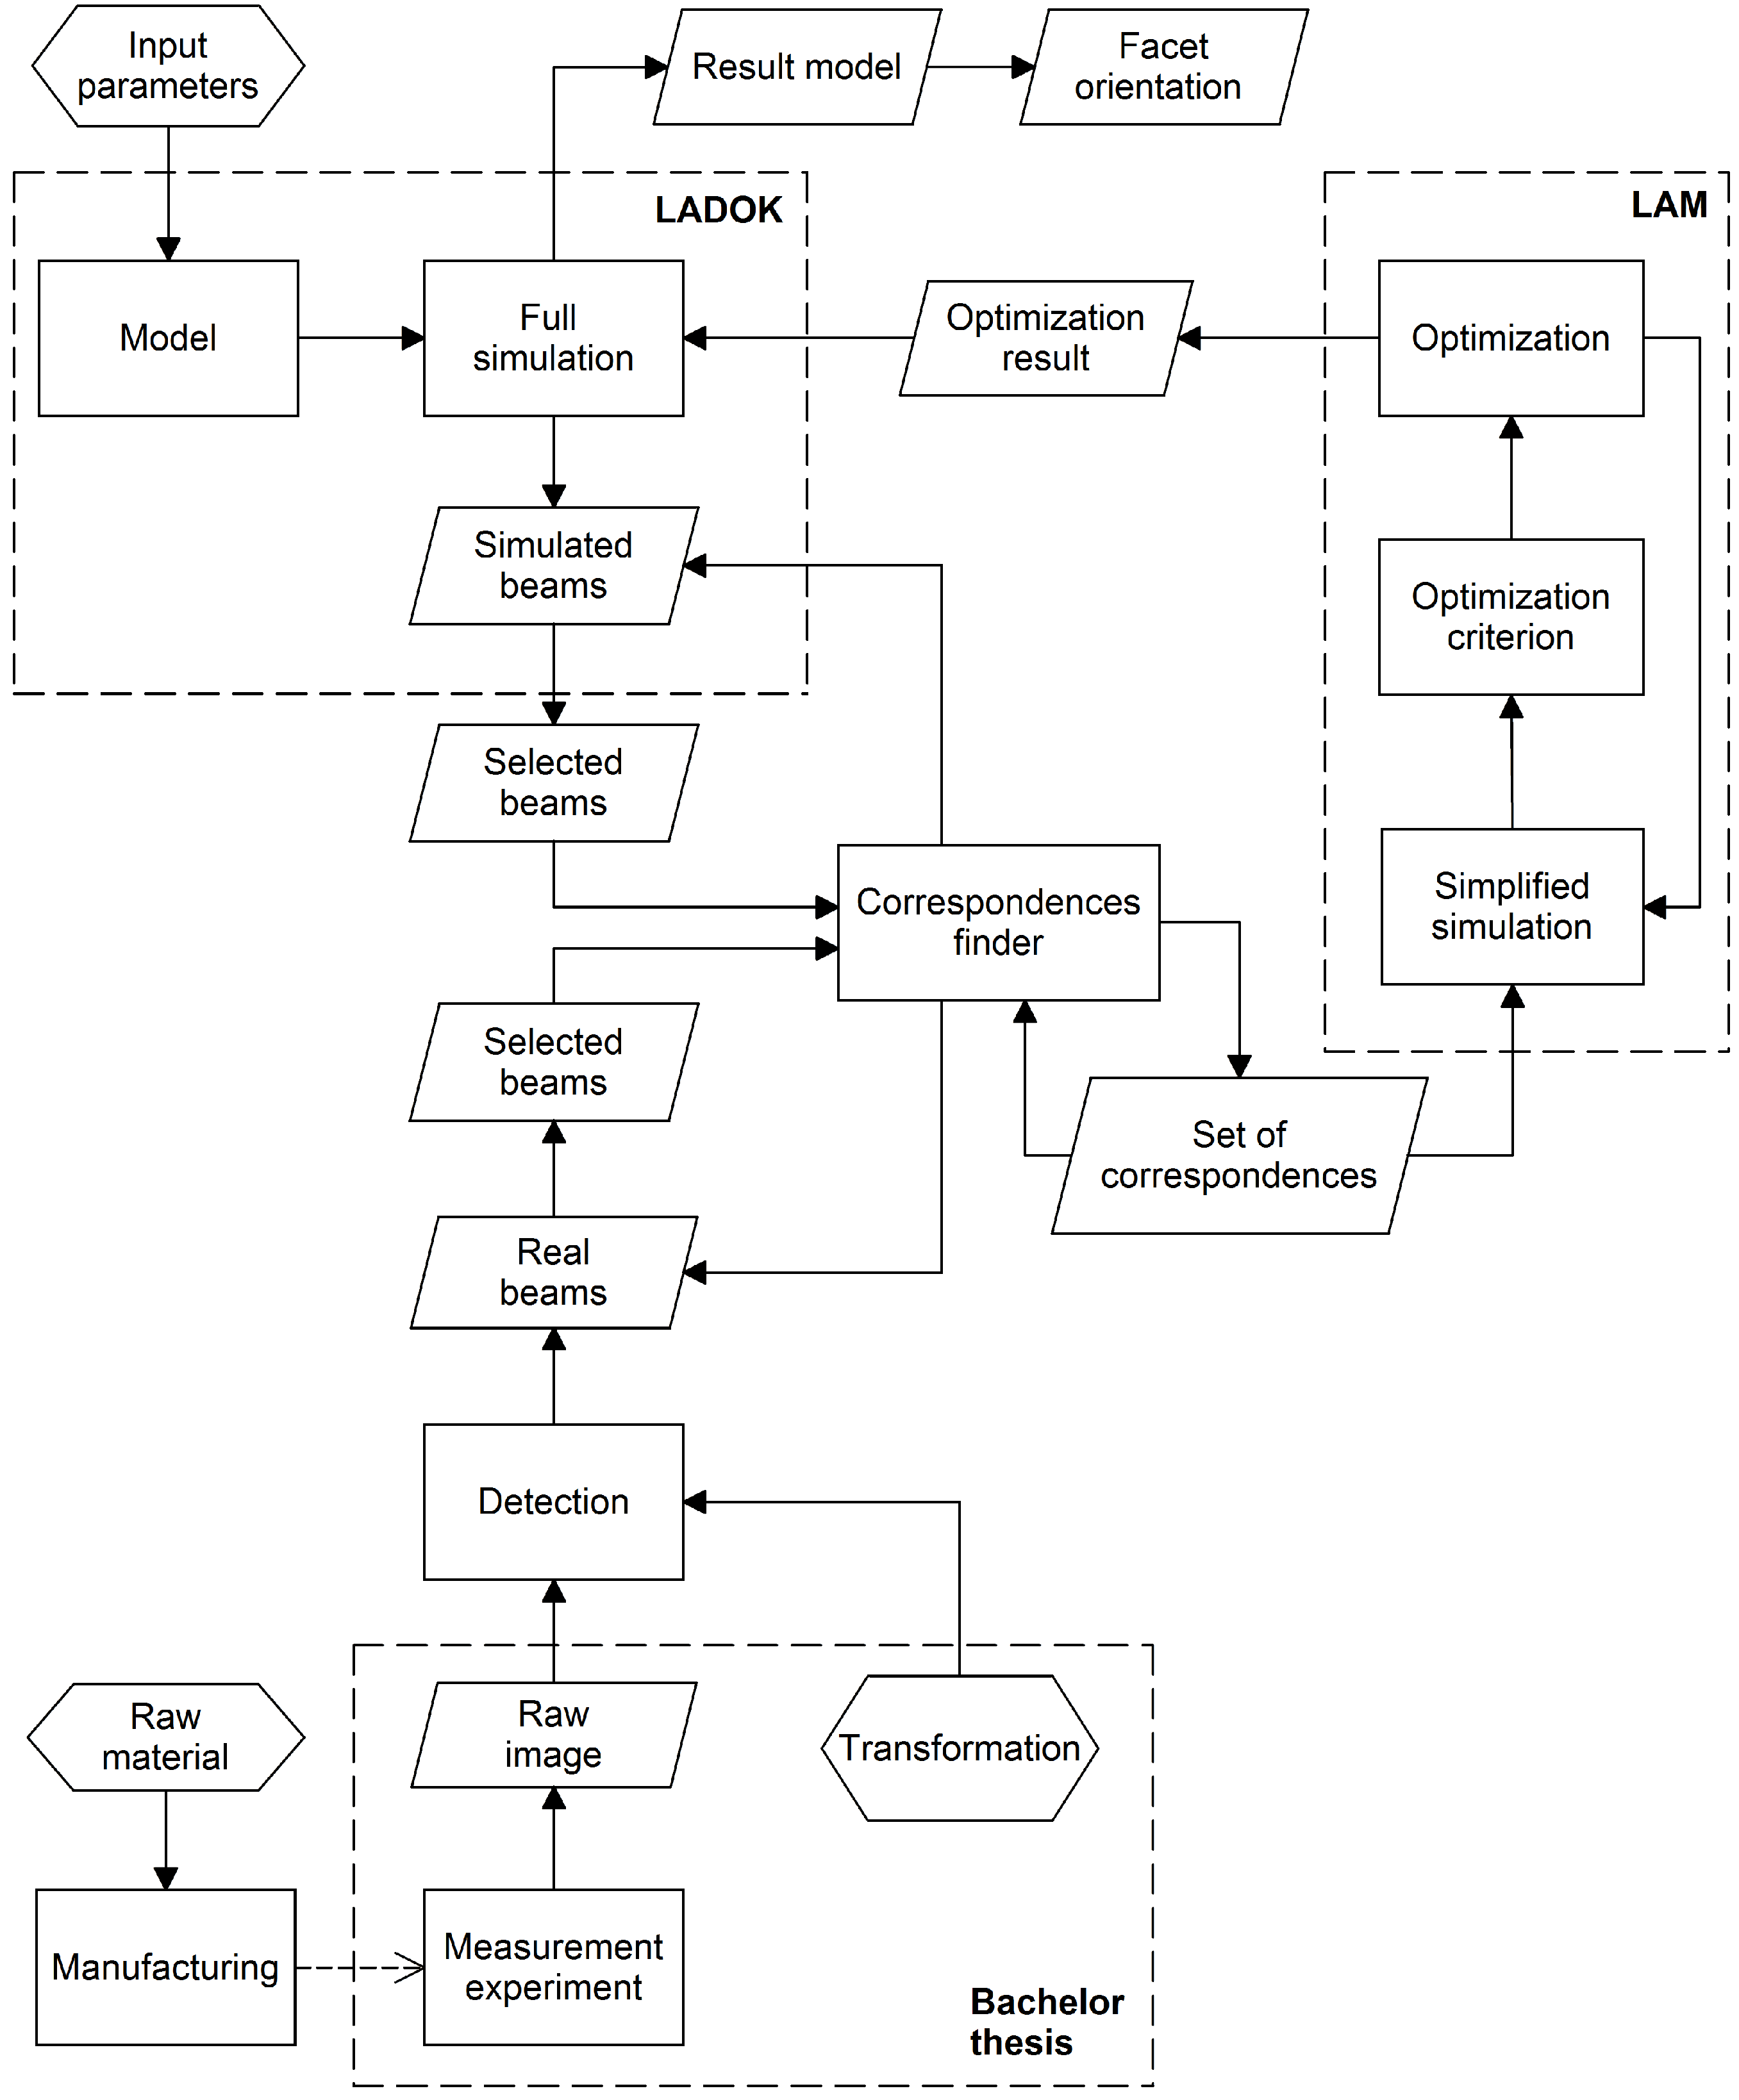
\includegraphics[width = 0.85\textwidth]{diagram.eps}
\caption{Diagram s principem odhadu orientace faset broušených kamenů.}
\label{fig:diagram}
\end{figure}

\clearpage


\section{Optimalizované kritérium}
\label{sec:Optimalizace_crit}
Optimalizační algoritmus je převzat z práce \cite{Bodlak2005}. Na rozdíl od LAMu využíváme optimalizační algoritmus nejen k odhadu parametrů faset kamene, ale také k odhadu indexu lomu kamene a jeho orientace v měřicí soustavě.

Definujeme kriteriální funkci, kterou budeme optimalizovat. Funkci lze popsat vztahem 

\begin{equation}
\vec{\varepsilon} = h\left(\vec{x},\vec{v},\vec{l},\vec{p} \right)\,.
\label{eq: opt_criter}
\end{equation}

\begin{tabular}{l p{12cm}}
$\vec{x}$ & Vektor parametrů, které nastavuje optimalizační algoritmus.
\paragraph{Parametry faset, index lomu}
\hspace{1mm}

 Jedná se převážně o parametry $r$ uvolněných faset. Každou fasetu lze parametrizovat pomocí úhlové změny normálového vektoru $\vec{n}$ (2 parametry) a změny vzdálenosti $d$ fasety od souřadného systému (1 parametr).\\
& Optimalizační metoda nemá dostatečnou citlivost na změny vzdálenosti $d$ fasety \cite{Bodlak2005}. Tento parametr proto považujeme za konstantu.\\
& Nově lze mezi optimalizované parametry přidat index lomu kamene $n_i$. Celkově máme $2\,r + q$ parametrů, kde $q$ je 1 pokud je mezi $\vec{x}$ parametr $n_i$, jinak je $q$ rovno 0.

\paragraph{Orientace} 
\hspace{1mm}

Orientaci kamene popisujeme rotací kolem vertikální osy $R_z$ a dvou parametrů definujících náklon kamene $R_x$, $R_y$. 
 \\ & \\
 
$\vec{v}$ & Popisuje směr zdrojového svazku světla.\\ & \\  

$\vec{l}$ & Obsahuje pole seznamů dopadových faset svazků. Seznam je využit pro výpočet směru výstupního svazku. Délka pole musí být rovna $s$. \\ & \\
 
$\vec{p}$ & Obsahuje směrové vektory pozorovaných svazků. Směr popisujeme pomocí souřadnic azimutu a elevace. Pokud pro výpočet optimalizačního kritéria použijeme $s$ pozorovaných svazků, bude mít vektor $\vec{p}$ délku $2s$. \\ & \\

$\vec{\varepsilon}$ & Představuje vektor odchylek v elevaci a azimutu simulovaných a pozorovaných svazků.\\ 
& V práci \cite{Bodlak2005} byla tato odchylka měřena jako chyba v pozici dopadu laserového svazku na stínítku. Důvodem proč bylo využíváno toto kritérium byla citlivější odezva při změně vektoru svazku. Hlavním důvodem volby azimutu a elevace pro výpočet optimalizačního kritéria v této práci je rychlost výpočtu. Odpadá totiž potřebný výpočet, který transformuje směrový vektor do souřadnic na stínítku. Vektor $\vec{\varepsilon}$ má $2s$ prvků.\\ & \\

\end{tabular}

\newpage

\section{Plná vs. zjednodušená simulace}
V optimalizačním cyklu je použito dvou simulací, které simulují průlet světla broušeným kamenem.

\subsection{Plná simulace}
Plnou simulací rozumíme klasický program LADOK, který modeluje odraz a lom svazků v konvexním tělese. Nevýhodou algoritmu je ale to, že simulace trvá příliš dlouho na to, aby mohla být úspěšně použita v optimalizačním procesu.

\paragraph{Časová náročnost simulace v LADOKu}
\hspace{1mm}

	U matematická simulace programu LADOK můžeme nastavit do jaké hloubky budou simulovány výstupní svazky. Při řešení se můžeme omezit na svazky s maximálním počtem dopadových faset $n_d$. V grafu \ref{fig: ladok_time} je zakreslena časová závislost programu LADOK při výpočtu simulovaných svazků kamene \textit{viva12} po různý počet dopadových faset. 
	
	\begin{figure}[htbp]
    \centering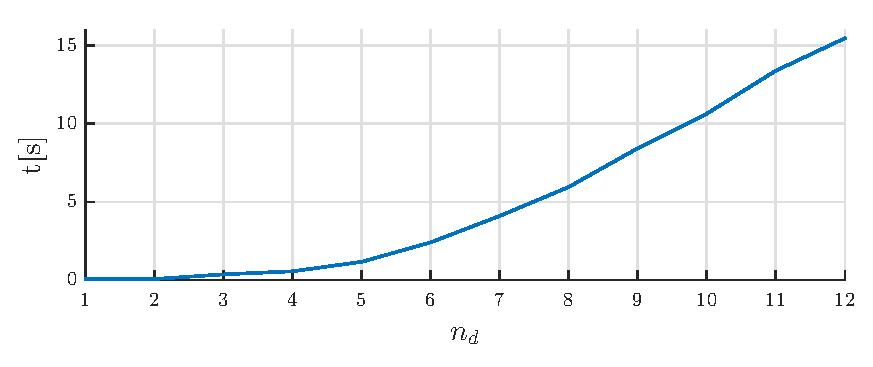
\includegraphics[width=0.7\textwidth]{ladok_time.eps}
     \caption[Časová náročnost simulace LADOK.]{Výpočetní doba simulace simulovaných svazků v programu LADOK v závislosti na počtu dopadových faset svazků.}
 \label{fig: ladok_time}
 \end{figure}

	
	Vzhledem ke strmému nárůstu časové náročnosti simulace programu LADOK budeme před každým výpočtem volit minimální $n_d$, tak abychom získali informace o všech simulovaných svazcích, které v dané situaci potřebujeme.      


\subsection{Zjednodušená simulace}
Základní myšlenkou vedoucí ke vzniku zjednodušené simulace je skutečnost, že se optimalizované parametry $\vec{x}$ při optimalizaci parametrů faset příliš nemění. Za tohoto předpokladu si podstatná část svazků zachová posloupnost dopadových faset. Vynecháme proto kontrolu vzniku či zániku svazků. 

Zjednodušená simulace vyřadí z plné simulace zbytečné výpočty, které v procesu optimalizace nevyžíváme. 
Jediné, co potřebujeme znát je směr výstupních svazků. Pro výpočet směru nahradíme svazky nekonečně tenkými paprsky a můžeme s nimi pracovat jako s vektory. Fasety kamene reprezentujeme pomocí normálového vektoru. 

Zjednodušená simulace přistupuje k paprsku jednotlivě. Funkci pro výpočet vektoru výstupního paprsku $\vec{v}_o$ lze vyjádřit jako  

\begin{equation}
\vec{v}_o= g\left(\vec{v}_i,\vec{N} \right)\,,
\end{equation}
kde $\vec{v}_i$ je vektor vstupního paprsku. Vektor $\vec{N}$ obsahuje normály $\vec{n}_1,\dots,\vec{n}_m$ faset na které svazek dopadá. Normály jsou seřazené v pořadí, které odpovídá dopadovým fasetám při šíření paprsku od zdroje ke stínítku. 

Při výpočtu musíme vědět, která faseta svazek odráží a která lomí. Situace je jednoduchá. Pokud $m = 1$, potom muselo dojít pouze k odrazu od fasety. Pokud  $m > 1$  odpovídají normály $\vec{n}_1$ a $\vec{n}_m$ fasetám, přes které se svazek lomí. Na ostatních fasetách se svazek odrazí. 

Zjednodušená simulace v LAMu navíc počítá polohu, kam paprsek na fasetu dopadl. Výpočet polohy paprsku byl kvůli rychlosti výpočtu odstraněn.



\section{Podmíněnost}
Základní otázkou optimalizačního problému je, zda úloha dostatečně podmíněná. První podmínku, kterou musíme splnit je získat minimálně stejný počet nezávislých rovnic, jako je počet optimalizovaných parametrů. 

V optimalizačním kritériu máme celkem  $2\,r + q$ nezávislých rovnic. Základní podmínkou je, že počet korespondujících svazků musí být minimálně $ s+q $.

\subsection{Třída svazků \textbf{1A} a \textbf{1B}}
Od tříd \textbf{1A} a \textbf{1B} lze obecně čekat velmi dobrou podmíněnost. Jednotlivý svazek z těchto tříd dopadne pouze na jednu fasetu a směr odraženého svazku jednoznačně určuje parametry fasety, od které se svazek odrazil. Pokud by náš matematický model přesně odpovídal reálnému experimentu, potom postačí nalézt korespondence třídy \textbf{1A} a \textbf{1B}, abychom určili orientaci všech faset kromě spodku. Tyto třídy nepodmiňují index lomu kamene.
 
\subsection{Třída \textbf{3A}}
Korespondencí svazků třídy \textbf{3A} (např. UF1-TOP-BOT) získáme 2 rovnice $\Delta \varepsilon$ pro elevaci a $\Delta \alpha$ pro azimut, které jsou závislé na parametrech dopadových faset UF1, TOP a BOT. Problém spočívá v tom, že tato korespondence určuje pouze vzájemnou polohu dopadových faset a nelze u této třídy očekávat dobrou podmíněnost. 
Abychom mohli optimalizovat náklon faset, potřebujeme znát další třídy korespondencí. Vhodná může být např. třída \textbf{5D}, což se podrobněji dozvíme v kapitole \ref{sec: klin}.

\section{Pozorování}

\subsection{Vzájemná poloha svazků}
\label{sec: klin}
Simulujeme průlet světelného svazku optickým klínem (obr. \ref{fig:wedge}). Prostředí s indexy lomu $\eta_1$, $\eta_2$ a $\eta_3$ oddělují rozhraní $\rho_1$ a $\rho_2$. Tato rozhraní mezi sebou svírají úhel $\alpha$.
\begin{figure}[h!]
\begin{center}
\scalebox{0.725}{ \input{xfig/mirror2.pstex_t}}
\end{center}
\caption{Lom a odraz paprsku v optickém klínu.}
\label{fig:wedge}
\end{figure}

\begin{equation}
\gamma = \arcsin{\left(\frac{\eta_1}{\eta_2}\sin{\beta}\right)}\,.
\end{equation}

\begin{equation}
\varepsilon_1 = \arcsin{\left(\frac{\eta_2}{\eta_1}\sin{\left(\gamma + 2\,\alpha\right)}\right)}\, 
\rightarrow \begin{cases}
\alpha > 0, & \varepsilon_3 > \varepsilon_2 > \varepsilon_1 > \beta\\
\alpha = 0, & \varepsilon_3 = \varepsilon_2 = \varepsilon_1 = \beta\\
\alpha > 0, & \varepsilon_3 < \varepsilon_2 < \varepsilon_1 < \beta
\end{cases}
\end{equation}

\begin{tabular}{p{2cm} l}
$\eta_1$ & index lomu vzduchu,\\
$\eta_2$ & index lomu materiálu kamene,\\
$\eta_3$ & index lomu odrazivé vrstvy,\\
$\rho_1$ & tabulka,\\
$\rho_2$ & spodek,\\
\textbf{0} & zdrojový svazek,\\
\textbf{1} & svazek třídy \textbf{1B} - TOP,\\
\textbf{3} & svazek třídy \textbf{3B} - TOP-BOT-TOP,\\
\textbf{5} & svazek třídy \textbf{5E} - TOP-BOT-TOP-BOT-TOP,\\
\textbf{7} & svazek třídy \textbf{7H} - TOP-BOT-TOP-BOT-TOP-BOT-TOP,\\
\textbf{2,4,6,8} & tyto svazky nevznikají - na rozhraní $\rho_2$ dochází pouze k odrazu.\\
\end{tabular}
\vspace{2mm}

Svazek dopadá na rozhraní $\rho_1$ pod úhlem $\beta$. Na obrázku \ref{fig:wedge} je tento svazek reprezentován paprsek č. 0. 

Svazek světla můžeme charakterizovat velikostí zářivého toku $\phi_e$. Z Fresnelových rovnic \cite{Handbook} víme, že pokud na rozhraní $\rho_1$ nedochází k totálnímu odrazu, tak po dopadu svazku na rozhraní vznikne odražený a lomený svazek. Jaká bude velikost zářivého toku odraženého svazku $\phi_{e_{reflect}}$ závisí na polarizaci světla, dopadajícím úhlu a poměrem mezi indexy lomu prostředí, které odděluje rozhraní $\rho_1$.

\begin{equation}
\phi_e = \phi_{e_{reflect}} + \phi_{e_{refract}}\,.
\end{equation}

 Při dopadajícím úhlu $\beta = 0^\circ$ a indexech lomu $\eta_1 = 1$, $\eta_2 = 1.5$ se \SI{4}{\percent} dopadajícího zářivého toku odrazí. $\frac{\phi_{e_{reflect}}}{\phi_e} = 0.04$, $\frac{\phi_{e_{refract}}}{\phi_e} = 0.96$.

Z principu šíření světla optickým prostředím pozorujeme svazky 0 až 9, se specifickým směrem šíření. 

V šatonové růži nastává stejný optický jev mezi tabulkou (TOP) a spodkem (BOT). V reálné situaci nejsou fasety TOP a BOT rovnoběžné. Důsledkem toho svazky \textbf{1B}, \textbf{3B}, \textbf{5E} a \textbf{7H} svírají s normálou tabulky různý úhel. Svazek třídy \textbf{3B} bude mít vždy největší zářivý tok. Zajímavé je, že tyto svazky leží ve stejné rovině. Tato rovina je určena vzájemnou orientací mezi normálou tabulky a normálou spodku.


\begin{figure} [h!]
\centering
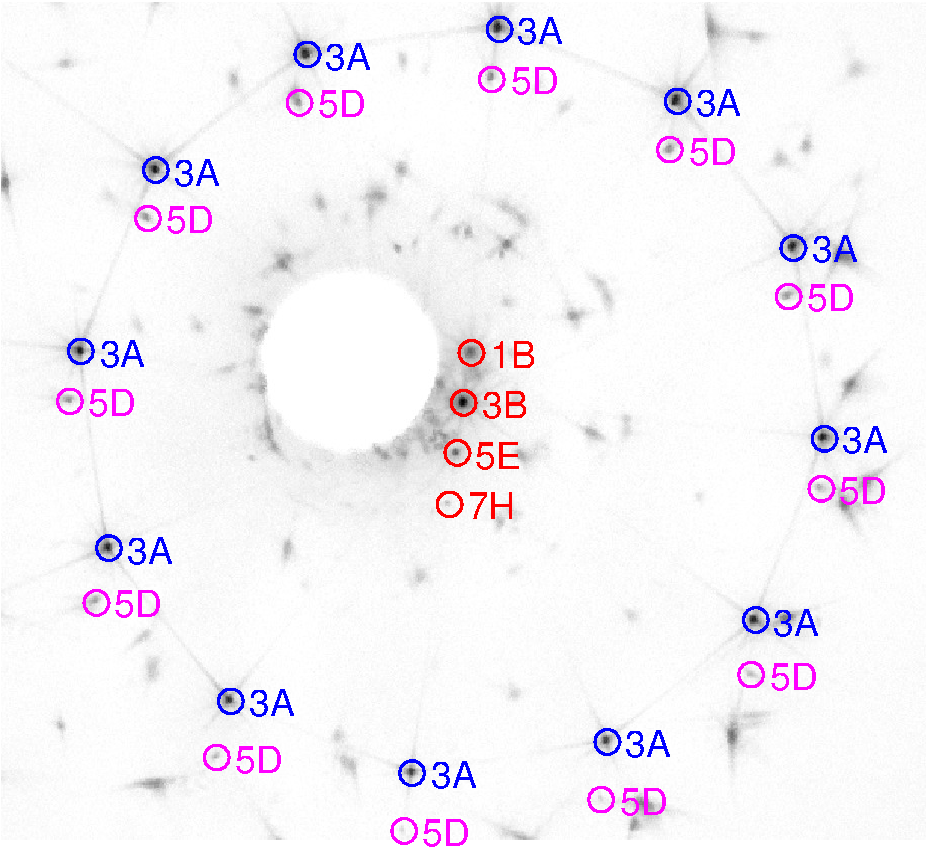
\includegraphics[width = 0.9\textwidth]{wedge_example.pdf}
\caption[Obrazy svazků ve snímku.]{Zvýraznění obrazů svazků ve snímku. Svazky třídy \textbf{1B}, \textbf{3B}, \textbf{5E} a \textbf{7H} dopadají pouze na fasetu TOP a BOT. Svazky třídy \textbf{3A} a \textbf{5D} dopadnou nejprve na boční fasetu a poté následuje jeden resp. dva dopady na dvojici faset BOT-TOP.}
\label{fig:wedge_example_image}
\end{figure}

\newpage
Dopad svazků  \textbf{1B}, \textbf{3B}, \textbf{5E} a \textbf{7H} na stínítko můžeme pozorovat na obr. \ref{fig:wedge_example_image}. Pokud bychom byli schopni přiřadit alespoň 2 tyto stopy ke svazkům můžeme určit orientaci tabulky a spodku. Situaci ovšem komplikuje fakt, že ne vždy můžeme nalézt obrazy těchto svazků, protože jsou často zastíněny podstavcem, na který pokládáme měřený kámen. 
 
 U svazků třídy \textbf{3A} a \textbf{5D} dochází k podobnému optickému jevu pouze s tím rozdílem, že svazek do kamene nevstupuje tabulkou, ale boční fasetou. Dvojice svazků třídy \textbf{3A} a \textbf{5D} se stejnou první dopadovou fasetou leží v jedné rovině.  Tato dvojice určuje vzájemnou orientaci mezi normálou tabulky a normálou spodku. Pro jednoznačné určení této orientace je však nutné znát orientaci bočních faset.  


\subsection{Orientace kamene}
Kámen je do měřicí soustavy umístěn ručně tak, aby se vertikální osa kamene nacházela v těžišti dopadajícího zdrojového svazku. Takto je zajištěna poloha kamene, ovšem rotace kamene okolo vertikální osy může být libovolná. 

Podle plochy, na kterou pokládáme kámen nemůžeme automaticky určit orientaci fasety BOT. Podstavec není pevně přichycen a mezi fasetou BOT a podstavcem je nanesena řada vrstev. Pokud nejsou tyto vrstvy naneseny rovnoměrně je kámen v měřicí soustavě nakloněn.

Rotace a náklon kamene musí být nalezeny před optimalizací parametrů faset. 



\subsection{Zakřivení faset} 

Kameny se brousí rovinnými brusnými kotouči, proto předpokládáme, že fasety jsou ideálně rovné a lze je popsat pomocí normály. Svazky nemusí dopadat na celou plochu fasety, ale pouze na vymezenou část fasety. Pokud dochází k zakřivení fasety, může se normála popisující tento element plochy lišit od normály fasety. Zakřivení fasety kamene vzniká především kvůli pružnému uchycení kamene při broušení.

Pokud vzdálenost fasety od souřadnicového systému klesne, zvýší se plocha fasety. Plocha sousedních faset naopak klesne. Řada svazků dopadá pouze na okraj faset. Posun fasety doprovází změna zářivého toku některých svazků, které mohou i zcela zaniknout.

Zakřivenou fasetu můžeme aproximovat jako část kulové či válcové plochy s vysokým poloměrem křivosti. 
  
Pozorujeme vliv vzdálenosti fasety od souřadnicového systému na změnu zářivého toku svazků (viz kapitola \ref{sec: zmena_tok }). K~výrazné změně dochází především u svazků s nízkým zářivým tokem. Při posunu fasety dochází ke změně zářivého toku svazků, které jsou omezeny minimálně jednou hranou posouvané fasety. 

V současné době nedokážeme vliv vzdálenosti rozlišit. Je ale možné, že informace o změně zářivého toku se vzdáleností fasety může v budoucnu vést ke vzniku vhodné metody, pomocí které určíme vzdálenost fasety. 

\newpage
\subsection{Svazky s vysokou citlivostí}

Existují svazky, které dopadají na fasetu pod téměř kritickým úhlem, např. svazek na obr. \ref{fig: kritOdrazSvazek}. Výstupní směr těchto svazků je vysoce citlivý na sklon fasety. Tyto svazky dobře určují sklon elementu plochy fasety, na kterou dopadají. Pokud je faseta zakřivená, mohou tyto svazky negativním způsobem ovlivnit optimalizované kritérium, což ve výsledku vyústí k nežádoucímu sklonu fasety a oddálení korespondujících svazků dopadajících na jinou část plochy fasety. Tento problém by mohl být odstraněn s použitím vhodnější parametrizace faset.

\begin{figure}[htbp]
    \centering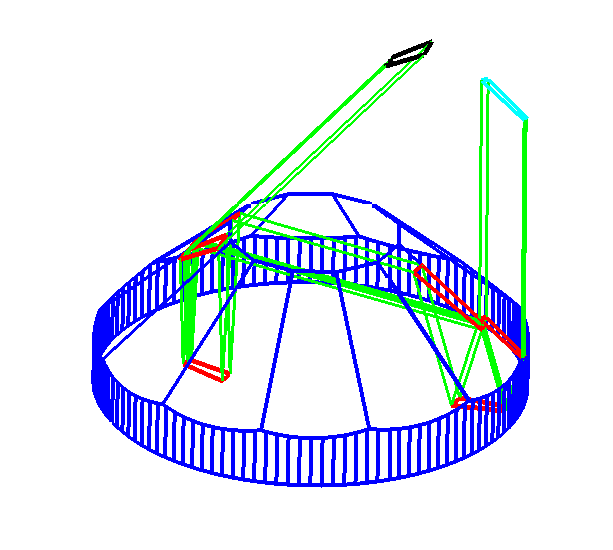
\includegraphics[width=0.5\textwidth]{svazek_krit_odraz2.eps}
     \caption[Svazek blízko kritického úhlu.]{Svazek třídy \textbf{6B}. Na poslední fasetu dopadá blízko kritického úhlu, proto je citlivější na sklon fasety než většina ostatních svazků.}
 \label{fig: kritOdrazSvazek}
 \end{figure}
 
 
 \clearpage